\PassOptionsToPackage{usenames, dvipsnames}{xcolor}
\documentclass[tikz, 10pt]{standalone}
\usepackage{fontspec}
  \defaultfontfeatures{Ligatures={NoCommon, NoDiscretionary, NoHistoric, NoRequired, NoContextual}, Mapping=tex-text}
  \setmainfont{Times New Roman}
\usepackage{xcolor}
\usepackage{graphicx}
\usepackage{relsize}
\usepackage{tikz, tikz-qtree}
	\usetikzlibrary{shapes, arrows, backgrounds, fit, positioning}

\begin{document}
  \begin{tikzpicture}[node distance=4em, anchor=west, align=flush center, FLOW/.style={->, very thick}, LABEL/.style={draw, fill=yellow!80, inner sep=.75em}, scale = 2, transform shape]
  	\node{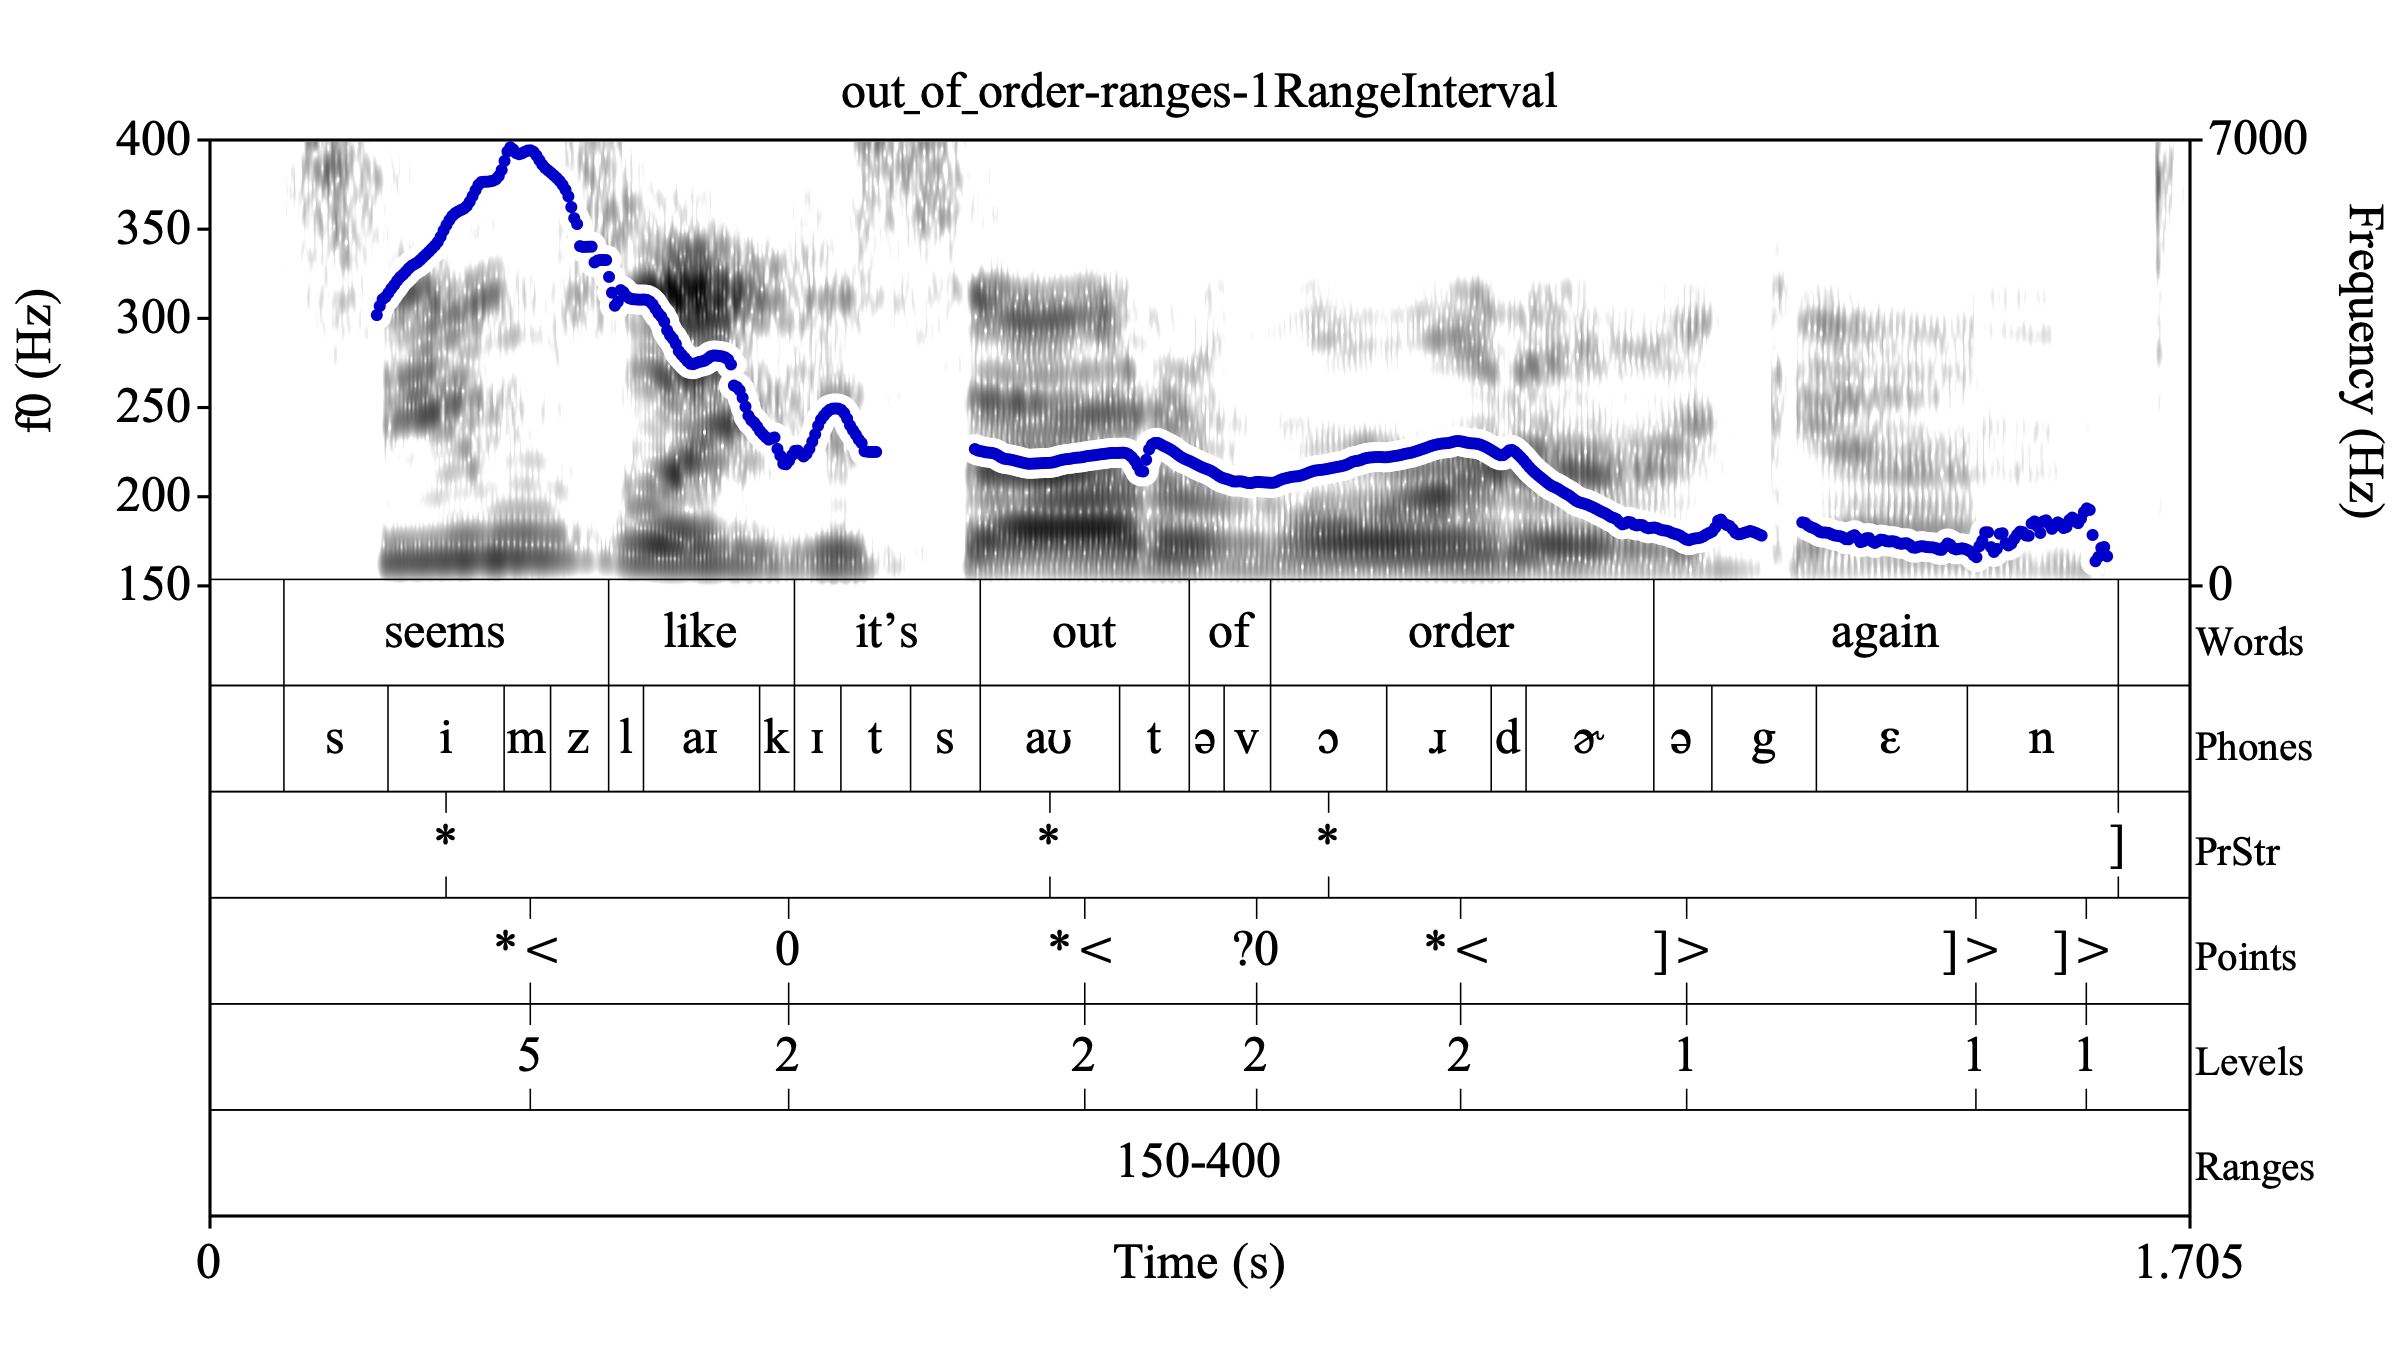
\includegraphics[width=25em]{Ranges-out_of_order-ranges-1RangeInterval.png}};
    \draw [black, fill=violet!30, opacity=.5] (1, 0.35) rectangle (8, 0.67);
    \draw [black, fill=blue!30, opacity=.5] (1, 0.67) rectangle (8, 0.99);
    \draw [black, fill=green!30, opacity=.5] (1, 0.99) rectangle (8, 1.31);
    \draw [black, fill=yellow!30, opacity=.5] (1, 1.31) rectangle (8, 1.63);
    \draw [black, fill=red!30, opacity=.5] (1, 1.63) rectangle (8, 1.95);
	\draw[red, opacity=.35] (2.065, -1.2) -- (2.065, 1.95);
	\draw[red, opacity=.35] (3.01, -1.2) -- (3.01, 1.95);
%	\draw[red, opacity=.35] (3.25, -1.2) -- (3.25, 1.625);
	\draw[red, opacity=.35] (4.1, -1.2) -- (4.1, 1.95);
	\draw[red, opacity=.35] (4.73, -1.2) -- (4.73, 1.95);
	\draw[red, opacity=.35] (5.47, -1.2) -- (5.47, 1.95);
	\draw[red, opacity=.35] (6.3, -1.2) -- (6.3, 1.95);
	\draw[red, opacity=.35] (7.36, -1.2) -- (7.36, 1.95);
	\draw[red, opacity=.35] (7.76, -1.2) -- (7.76, 1.95);
%	\draw[step=.5, black] (2, 0) grid (8, -2);
  \end{tikzpicture}
\end{document}